\documentclass{article} % For LaTeX2e
\usepackage{nips13submit_e,times}
\usepackage{hyperref}
\usepackage{url}
\usepackage{graphicx}
\usepackage{amsmath}
\usepackage{amsfonts}
\usepackage[ruled,vlined]{algorithm2e}
%\documentstyle[nips13submit_09,times,art10]{article} % For LaTeX 2.09


\title{Predicting Popularity of YouTube Video}

\author{
Loc Do \\
Heinz College,
Carnegie Mellon University \\
Pittsburgh PA, 15213\\
\texttt{halocd@andrew.cmu.edu} \\
\And
Joseph Richardson \\
School of Computer Science,
Carnegie Mellon University \\
Pittsburgh PA, 15213 \\
\texttt{jmrichar@andrew.cmu.edu} \\
}

\newcommand{\fix}{\marginpar{FIX}}
\newcommand{\new}{\marginpar{NEW}}

\nipsfinalcopy % Uncomment for camera-ready version

\begin{document}

\maketitle

\begin{abstract}
	In this work we address the problem of ranking two objects given their features. The problem is applied to a context of guessing the more popular of two given YouTube videos. We formulate this problem into two different approaches, namely binary classification and linear regression. Experiments are conducted in our data set crawled from YouTube over a one-month span. Results show that both approaches yield a slightly above 50\% accuracy. We conclude that bag-of-words features with linear classifiers are not efficient in determining videos' popularity.
\end{abstract}

\section{Introduction}
\label{sec:intro}
	YouTube is one of the most popular video-sharing online platform in the Internet. It attracts billion of unique user visit monthly and had content for a wide variety of topics. YouTube users can earn money from the number of views of their uploaded videos. Hence, understanding the secrets of making a popular YouTube video is essential for people who want to use YouTube professionally. There are many factors to determine popularity of a video, but in general we can reduce them down to having good content and a good marketing plan. One of the techniques to attract more views is to make the video's "visual appearance" look appealing via catchy keywords, informative cover picture, etc.

	The ranking problem (aka. Learning to rank\footnote{http://en.wikipedia.org/wiki/Learning\_to\_rank}) is a typical supervised learning problem of predicting the rank of a set of items regarding some set of criteria. It has a numerous applications in a broad domains such as web search, multimedia retrieval, recommender systems, etc. Results from such problems can bring benefits to Internet users, such as saving their time by introducing only the content most relevant to their interests. In YouTube context, ranking problems arise in recommending the most relevant videos to a given video. Another application is to rank video popularity overall.

	\textbf{Problem statement.} Given a set of videos, each is associated with a set of bag-of-word and numeric features extracted from their metadata. We use the number of views as our measure of popularity. Given two videos with their features, the video ranking problem is to construct a model to accurately predict which one has more views.  In order to do this, we approach the problem in two different manners:  Ranking by classification, and ranking by regression.

\section{Ranking by Classification}
\label{sec:ranking}
	\subsection{Ranking as Logistic Regression}
We can reformulate the ranking prediction problem between two videos as a binary classification problem. To be specific, let $X_i \in \mathbb{R}^D$ and $X_j \in \mathbb{R}^D$ be feature vectors of two video $i$ and $j$ correspondingly. Each video pair $(i, j)$ is associated with a binary label $Y_{ij}$ defined as follows
\begin{equation}
	Y_{ij} = \begin{cases}
			   1, & \text{if } \text{\#\_of\_views\_i} \geq \text{\#\_of\_views\_j} \\
			   0, & \text{otherwise}
			\end{cases} 
\end{equation}	
 We can form a representative vector of the pair $(i, j)$ as follows
\begin{equation}
	\mathcal{X}_{ij} = k (X_i, X_j),
\end{equation}
where $k: (\mathcal{R}^D, \mathcal{R}^D) \rightarrow \mathcal{R}^{D'}$ is a feature transformation function. There are several options for $k$. 
\begin{itemize}
	\item Difference between two feature vectors: $\mathcal{X}_{ij} = X_i - X_j$
	\item Concatenation of two feature vectors:  $\mathcal{X}_{ij} = [X_i, X_j]$ (Matlab notation)
	\item Kernel functions, e.g. $\mathcal{X}_{ij} = || X_i - X_j ||^2$
\end{itemize}
At the moment, we cannot find any theories/signals to indicate which form of $k$ is the most appropriate. For the scope of the project, we choose to represent $X_{ij}$ as difference between $X_i$ and $X_j$, meaning $D = D'$. The kernelized version is left in future work. 

The function form of classifier $P(Y_{ij}|\mathcal{X}_{ij}, \textbf{w})$ as follows
 \begin{equation}
	 P(Y_{ij}=1|\mathcal{X}_{ij}, \textbf{w}) = \frac{1}{1 + \exp ( w_0 + \sum_d w_d \mathcal{X}_{ij}^d )} = \frac{1}{1 + \exp (\textbf{w}^T \mathcal{X}_{ij})}
 \end{equation}
 
The model parameters $\textbf{w} \in \mathbb{R}^D$ can be learnt using MAP.
\begin{align}
	\label{eqn:objFuncLR}
	\hat{\textbf{w}}_{MAP} &= \operatorname*{arg\,max}_{\textbf{w}} \prod_{(i,j)} P(Y_{ij}| \mathcal{X}_{ij}, \textbf{w}) P(\textbf{w}) \hspace{1 cm} \text{($P(\textbf{w}) \sim \mathcal{N} (0, \tau^2 I) $)}\\ \notag
	&= \operatorname*{arg\,max}_{\textbf{w}} \prod_{\{(i,j)|Y_{ij}=1\}} P(Y_{ij}| \mathcal{X}_{ij}, \textbf{w}) P(\textbf{w}) \hspace{1 cm} \text{($Y_{ij} + Y_{ji} = 1, \mathcal{X}_{ij} = - \mathcal{X}_{ji}$)}\\ \notag
	&= \operatorname*{arg\,max}_{\textbf{w}} \sum_{\{(i,j)|Y_{ij}=1\}} ln P(Y_{ij}| \mathcal{X}_{ij}, \textbf{w}) + ln P(\textbf{w}) \\ \notag
	&= \operatorname*{arg\,max}_{\textbf{w}} \sum_{\{(i,j)|Y_{ij}=1\}} ( (1 - Y_{ij})\textbf{w}^T\mathcal{X}_{ij} - ln(1 + \exp(\textbf{w}^T\mathcal{X}_{ij}))) - \lambda_w \|\textbf{w} \|^2_2 = l(\textbf{w})
\end{align}

We can optimise Equation \ref{eqn:objFuncLR} (a concave function) using Gradient Ascent with the following update rule
\begin{equation}
w^{t+1}_d \leftarrow w^t_d + \eta \frac{\partial l(\textbf{w})}{\partial w_d} = w^t_d + \sum_{\{(i,j)|Y_{ij}=1\}} \mathcal{X}_{ij}^d ( (1 - Y_{ij}) - \frac{\exp(\textbf{w}^T\mathcal{X}_{ij})}{1 + \exp(\textbf{w}^T\mathcal{X}_{ij})})  - \lambda_w w_d
\end{equation}

\section{Ranking by Regression}
\label{sec:regression}
	Another approach to the ranking problem is to predict the number of views for each video and then rank the videos based on predicted values, rather than comparing two videos directly. This approach has two advantages over the above approach of classification. First, it can take into account the magnitude of difference between two videos' viewership. Secondly, we can use it to predict a number of views of a video for a specific time in future given their current status. We treat this problem as an ordinary linear regression problem. 

\subsection{Problem Formulation}
Our linear function assumes that are labels $Y_i$ come from our input $X_i$ plus some noise $\epsilon$:
\begin{equation}
Y_u = X_u \beta + \epsilon,
\end{equation}
where $Y_i$ is the number of views of video $i$, $X_i$ is the associated feature vector. We therefore seek a function of the form
\begin{equation}
f(X) = X \beta
\end{equation}
and attempt to minimize the mean squared error loss function, giving
\begin{equation}
	\hat{\beta} = \operatorname*{arg\,min}_{\textbf{$\beta$}} 1/n (A \beta - Y)^T(A \beta - Y)
\end{equation}
where $A = [X_1 ... X_n]^T$ and $Y = [Y_1 ... Y_n]^T$, n is the number of training data points.

%We anticipated that this method will perform worse than logistic regression at the ranking problem.  However, this method, if successful, would have the added utility of allowing predictions on a video without needing to compare it to another.

In order to solve this problem, we can use either the closed form or Gradient Descent to learn the $\beta$ parameters.  However, since our feature space may be quite large, we opt for the latter.  We therefore initialize $\beta^0$ to 0, and thereafter use the update step
\begin{equation}
\beta^{t+1} = \beta^t - \eta A^T (A \beta^t - Y)
\end{equation}
 
Since our context is a bad conditioning problem, similarly to the Classification approach, we opt to Stochastic Gradient Descent with L2-Regularization. The new update function
	\begin{equation}
		\beta^{t+1} = \beta^t - \eta (x_i (x_i\beta^t - Y_i) + \beta^t)
	\end{equation}

After the learning stage is complete, the predicted ranking can be done as follows
\begin{equation}
\hat{Y}_{uv} = \mathbb{I}(\beta X_u > \beta X_v),
\end{equation}
where $\mathbb{I}$ is the indicator function, return 1 if the expression as argument is true, and 0 otherwise.

\subsection{Comparing Order-of-Magnitude}
\label{sec:orderofmagnitude}
	It is important to decide what we will consider as being "close to correct".  We use least-squared regression, where we minimize the total of the squares of the differences between our prediction and the true value.  However, we must deal with the gigantic variance in our observed data.

	Ideally, we wish to consider orders of magnitude rather than direct counts, and for this we will set our loss function equal to the square of the difference between the log of our prediction and the log of the observed value.  The motivation is that we wish to reflect the human intuition that there is more difference between the popularities of two videos with 10 and 1,000 views (respectively) than between two videos with 1,000,000 and 1,001,000 views.  This will prevent petty variations among the most popular videos from drowning out the differences in all others.

	We therefore deal with the number of views in log scale for the regression (though we also tried running our analysis without using log scale).  One anticipated effect of this is that features will be expected to contribute multiplicatively, rather than additively, to the popularity of a video.

\section{Experimental study}
\label{sec:experiment}
	\subsection{Dataset}
	We crawled and extracted our data from YouTube for one month (Oct - Nov, 2015). The crawling strategy is akin to bread-first search. First we initialize the crawler with several random "seed" videos, which mostly are in the \textit{Movie} and \textit{Music} category, and recursively explore all other related videos recommended by YouTube recommendation systems. For each video, we extract all of its metadata such as title, uploader and his number of subscriptions, description, upload date, number of views/likes/dislikes, video length, and a number of other attributes, as well as a list of around 30 videos YouTube recommends as being similar. 

	\subsubsection{Data Statistics}
		Although the crawler was suspended twice due to technical issues and upgrades, we have gathered a sizeable amount of data, with tremendous variation in the observed values:
		
		\begin{itemize}
			\item Number of videos crawled: 1,432,213
			\item Number of uploaders: 628,072
			\item Number of "bag of word" features (extracted from the titles): 2,447,603 entries
			\item Video length: $[1 \ldots 107,373]$ (seconds)
			\item Range of number of day passed since uploaded: $[1 \ldots 3423]$ (days)
			\item Range of number of views: $[7 \ldots 2,104,518,656]$.
			\item Range of number of likes: $[1 \ldots 8,639,650]$.
			\item Range of number of dislikes: $[1 \ldots 4,184,769]$.
		\end{itemize}

		We plot in Figure \ref{fig:histograms} different histograms reflecting characteristics of our data. In the red-colorer histogram, we look for the distributions of videos and their view counts. Interestingly, the distribution is in the shape of Gaussians, instead of following the Power Law distribution as frequently observed in social networks. We guess this observation is due to the way we sampled the data, by following the recommended links. It is intuitive since videos with high view counts are usually recommended together. The Gaussian distribution also encourages us to perform some standardisation on the data, such as subtracting the label to the mean of the Gaussian and predict the left amount. 
		

		\begin{figure}[!h]
			\begin{center}
				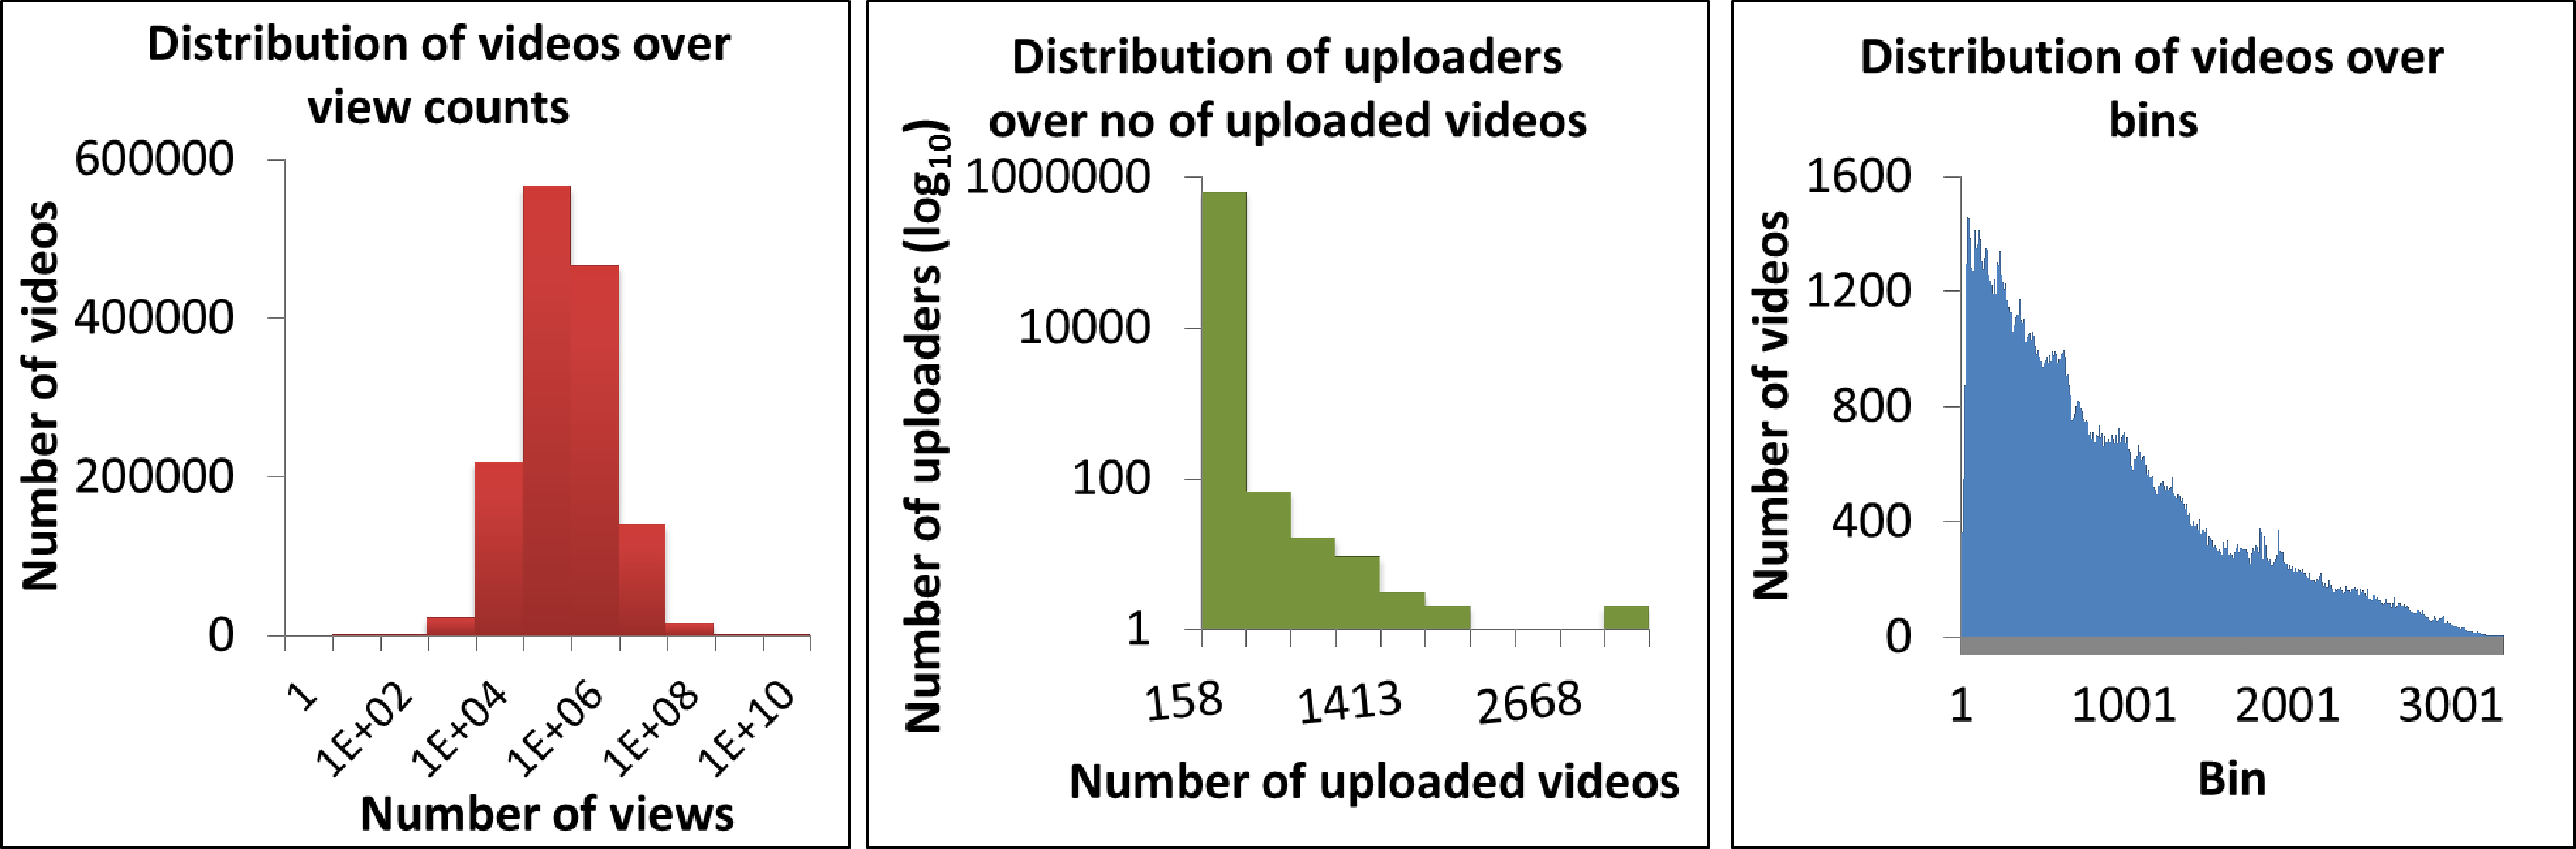
\includegraphics[width=1.0\textwidth,clip]{distributions.pdf}
			\end{center}
			\caption{Red-colored histogram: Distribution of videos over view counts. Blue-colored histogram: Distribution of uploaders over number of uploaded videos. Green-colored histogram: Distribution of number of videos in each bin.}
			\label{fig:histograms}
		\end{figure}
	
		As the statistics show, we have a large magnitude in ranges of number of view, likes and dislikes. This motivates us to do some preprocessing on data, such as feature normalization or data standardization, to ensure the numerical stability and good speed of convergence on the learning algorithm for logistic regression. We discuss more on this step in the Section \ref{sec:orderofmagnitude}.
						
	\subsubsection{Feature extraction}
		In this section we discuss the feature engineering process in the project. First, we build a dictionary mapping the uploader to the number of videos they have uploaded and the total number of views there videos have. We also take care to prevent "cheating":  In order to ensure that our predictor has only such information as would be available before the video's publishing is ever used, we temporarily reduce these number of video-views and the total number of video uploads for the uploader according to the publish date of the video under current consideration.

		We considered many features, which ultimately include:
		\begin{itemize}
			\item
			Features extracted via a bag-of-words model on the title, using TF-IDF.
			\item
			The number of videos uploaded by the uploader prior to the current video's upload date.  Because of our desire for caution against "cheating", we count only those videos that we have crawled.
			\item
			The total number of views for the uploader due to videos released prior to the current video's upload date.  Again, we count only those videos that we have crawled.  This date-conscious counting is particularly important because there are many cases where there is only one video crawled for a given uploader, meaning that this feature would become a nearly perfect predictor.
			\item
			The number of subscribers for the uploader.  We lack sufficient data to know how subscribers changed over time, so we simply had to keep this constant.
			\item
			The runtime of the video, in seconds.
			\item
			The age of the video at the time of crawling, in days.
			\item
			The number of likes/dislikes.  Since these are expected to scale with the number of views, we forbade ourselves from using the number directly, but we did allow certain combinations, such as the log of the like-vs-dislike ratio.
			\item
			Various combinations of the above features (for example, the log of some other feature, or the ratio between two features).
		\end{itemize}
	
\subsection{Evaluation Metrics}
	Normally, a rank correlation \footnote{http://en.wikipedia.org/wiki/Rank\_correlation} is a common metric in ranking problems. Since our problem is re-formulated as a classification and regression problems, we evaluate our methods using corresponding metrics such as Root Mean Square Error (RMSE) for Regression and $F_1$-score and Accuracy for Classification.
	
	\subsubsection{Classification}
	The error matrix (or confusion matrix) is a common way to measure performance of any arbitrary classifiers. Several metrics derived from this matrix are Accuracy, Precision-Recall, $F_1$-score or Receiver Operator Characteristics (ROC). In our work we employ two of them: Accuracy and $F_1$-score \footnote{http://en.wikipedia.org/wiki/F1\_score}.
	
	The accuracy can be equivalently stated as a 0-1 loss function over total number of pairs in testing set.
	\begin{equation}
		0/1_{loss} = \sum_{(u, v)_{test}} \frac{1}{|(u,v)_{test}|} \textbf{1}[\hat{Y}_{uv} - Y_{uv} == 0]
	\end{equation}
	
	\subsubsection{Regression}
	To Joseph: Can you put your least square formula here ? The first few paragraphs in section 4.3.2 can be put here. And show the equations as well.

\subsection{Results}
\label{sec:results}
	Due to our limitation in computing resources, we can only present our approaches for the first 30 bins (meaning videos with age ranging from 1 day to 30 days). For each bin, we create 5 folds cross-validation with 80\% of our data for training, and the other 20\% for testing. The average results over 5-folds are reported.

We set the learning rate $\eta=1$, $\lambda=0.01$. The maximum of iteration is $maxIter=3$. We did try with other values of $maxIter$ up to 10, but they do not give significant gains and take more time to run.

\subsubsection{Classification Results}
	The accuracy and $F_1$-score of our logistic regression are presented in Table \ref{tbl:acc} and Table \ref{tbl:f1} correspondingly. For each metric, we present four approaches: original logistic regression (ORG), logistic regression with augmented features (AUG), logistic regression with weighed gradients (GRAD) and logistic regression with both extensions (BOTH). Each approach we compare with its corresponding ensemble version as described in section \ref{subsec:ext2}. 
	
Although all the approaches return barely above 50\%, there are some observations. First, the extension with augmented features have better performance than original approach. Meanwhile, the other extension with weighted gradient shows less effective in prediction.  That makes senses since we put more weights on the gradients, we have to employ a better control on the learning rate. Otherwise the parameters would oscillate over the optimal points. It also explains the 'BOTH' method performs the worst in accuracy and $F_1$-scores.
	
Secondly, most of the ensemble methods have better performance (both in accuracy and $F_1$-scores) than single predictions. That supports our hypothesis that by partitioning the videos into bins, we worsen the sparseness in each bin's data. Hence by using an weighted combination of all classifiers, we can pass information between the bins to achieve better performance. Recall that the ensemble methods work only if all the individual predictors have good performance in their own data. Since 'BOTH' and 'GRAD' have lower accuracy in prediction, ensemble methods do not work in their cases. That explains the exceptional observations in $F_1$-scores when the single predictors of both perform better.
		
			\begin{table}[h]
			\caption{Average of Accuracy over 5 folds of 30 bins.}
			\label{tbl:acc}
				\begin{center}
					\begin{tabular}{| l | c | c |}						
					\hline
					Approach & Single Predictor & Ensemble \\ \hline
					BOTH & 0.513 & \textbf{0.526} \\ \hline
					GRAD & 0.514 & \textbf{0.527} \\ \hline
					AUG & 0.516 & \textbf{0.534} \\ \hline
					ORG & 0.514 & \textbf{0.532} \\ \hline		
					\end{tabular}
				\end{center}	
			\end{table}

	\begin{table}[h]
	\caption{Average of $F_1$-score over 5 folds of 30 bins.}
	\label{tbl:f1}
		\begin{center}		
			\begin{tabular}{| l | c | c |}
			\hline
				Approach & Single Predictor & Ensemble \\ \hline
				BOTH & \textbf{0.468} & 0.463 \\ \hline
				GRAD & \textbf{0.451} & 0.443 \\ \hline
				AUG & 0.473 & \textbf{0.503} \\ \hline
				ORG & 0.455 & \textbf{0.468} \\ \hline
			\end{tabular}
		\end{center}
	\end{table}
	
\subsubsection{Regression Results}
	The linear regression can be evaluated in more than one way.
	
	The first way to measure our results is to look at its predictions directly.  Our mean squared error indicated that our prediction was was typically 0.93 orders of magnitude away from the true result, but it is hard to say whether we should be impressed.
	
	The second form of evaluation is to compare the results for each pair of videos and then use the \textbf{0-1 loss function}, so that results can be compared to the logistic regression results.  Not surprisingly, logistic regression performed better (having been trained explicitly for this task).  What is surprising, however, is that our accuracy is not significantly greater than 50\%, which indicates that our linear regression holds no measurable value for the ranking problem.
	
	A likely cause is that this problem may not be linear in nature -- in fact, it would admittedly be surprising if it were.  We tested our accuracy on the training data as well as on the testing data, and found that it performed just as poorly, indicating that the weak results on our testing data did not stem from over fitting.
	
	In order to investigate further, we plotted our output against the true number of views (for a random subset of our data):

	\begin{figure}[!h]
		\begin{center}
			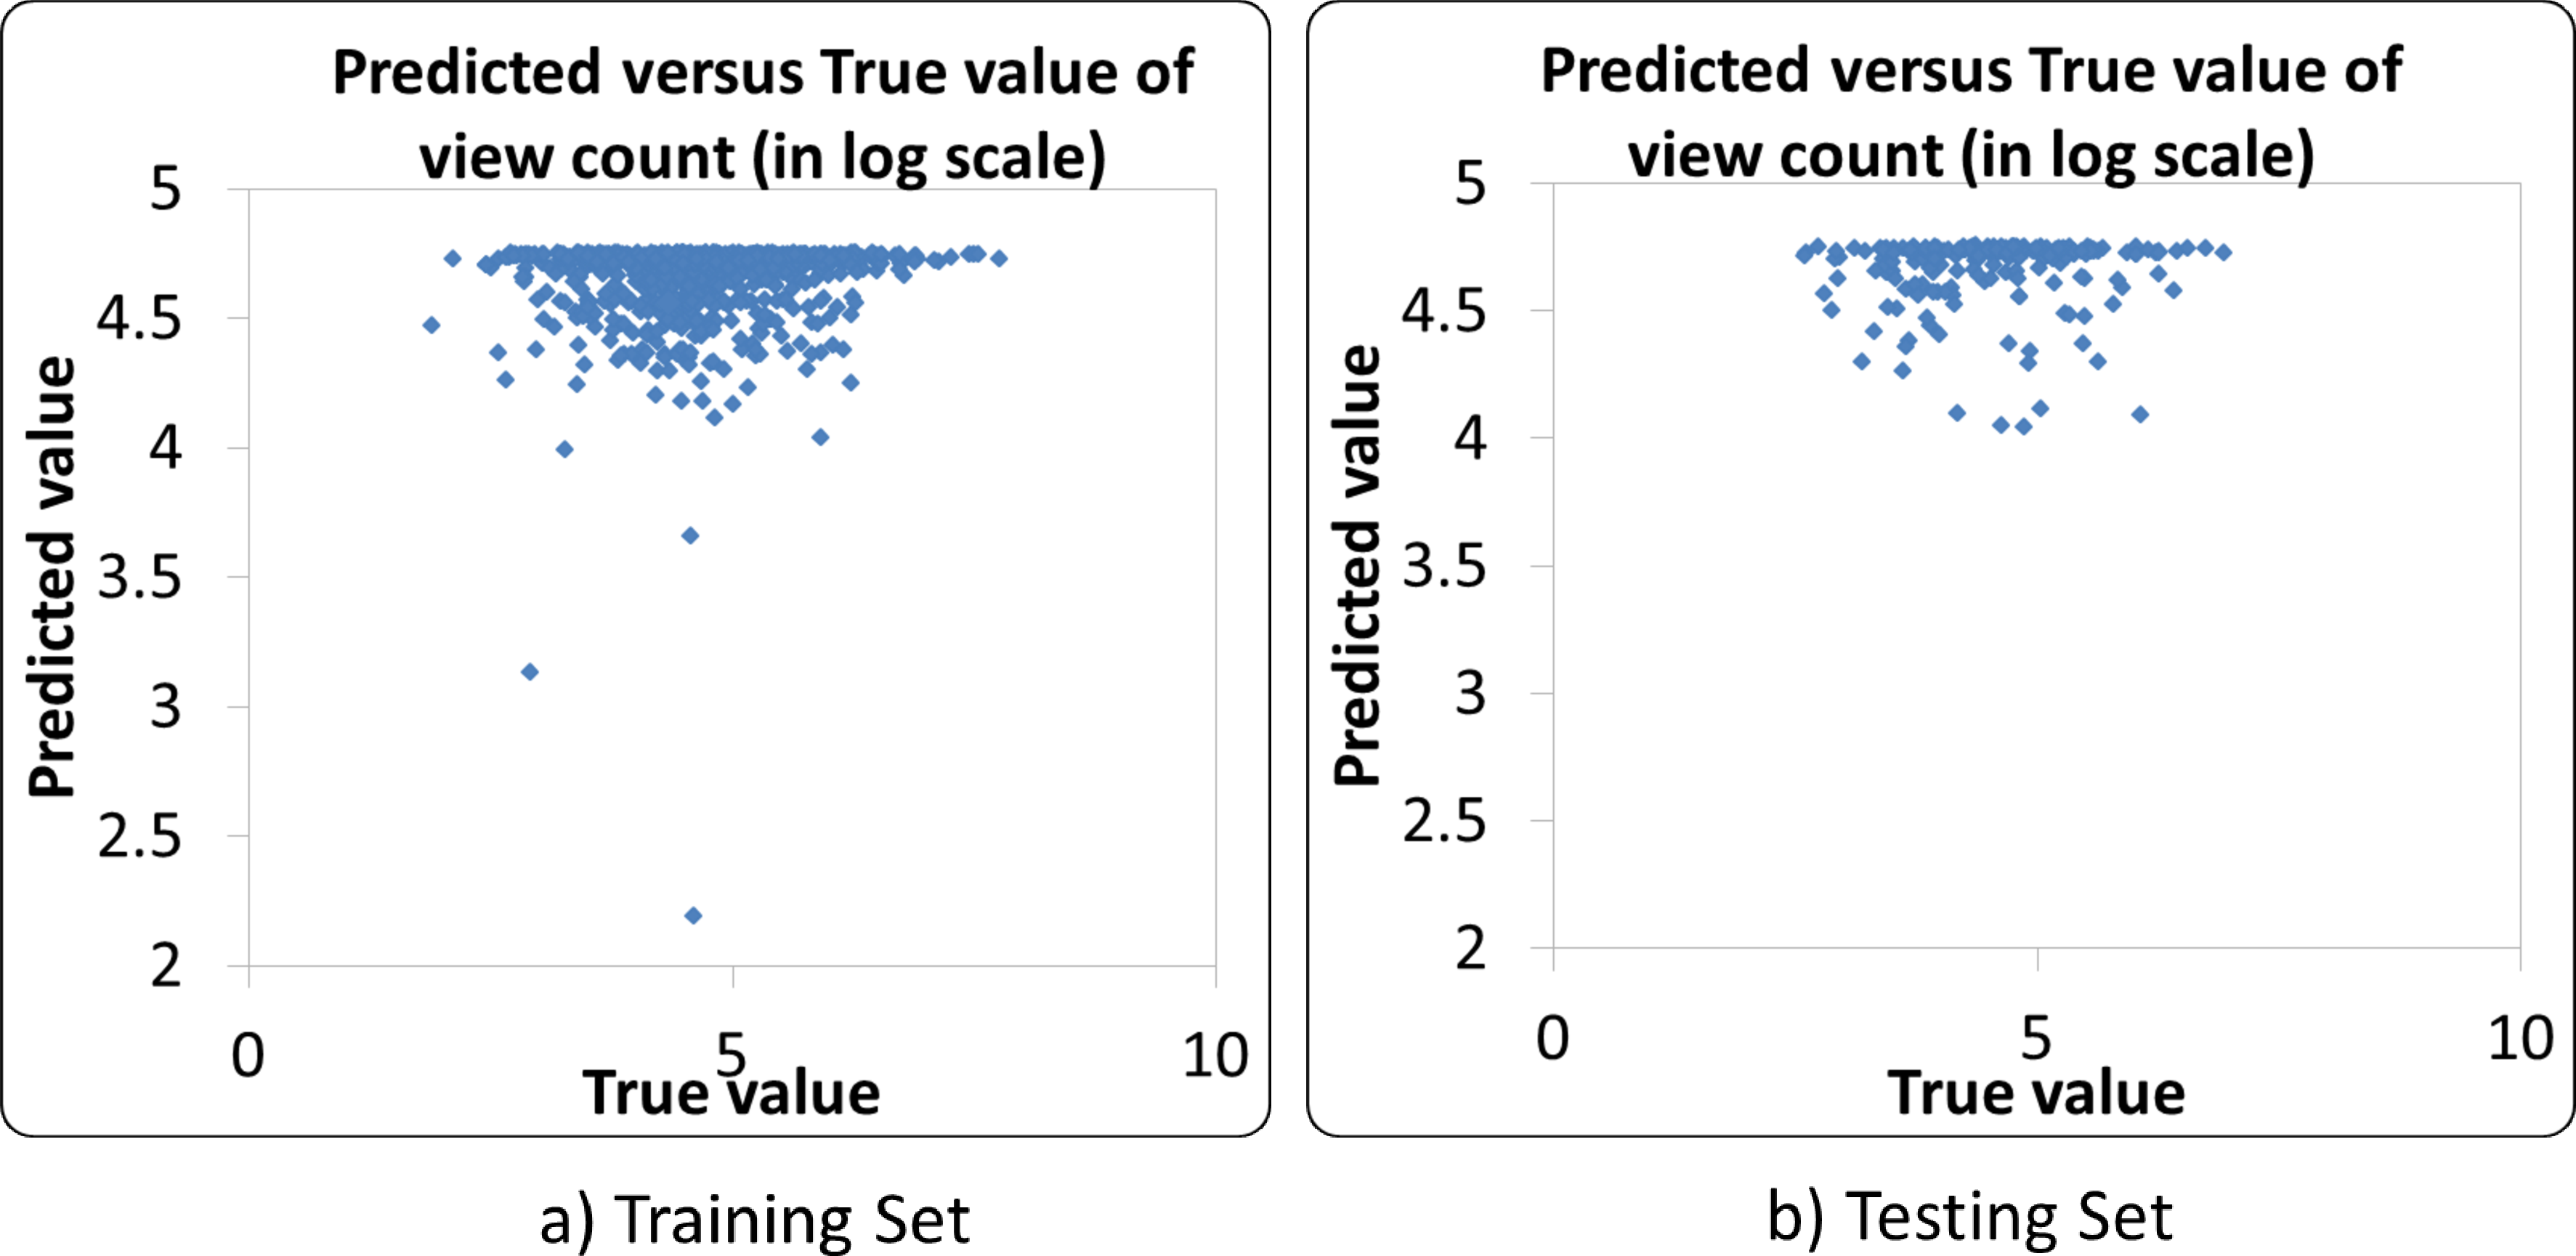
\includegraphics[width=.75\textwidth,clip]{regression.pdf}
		\end{center}
		\caption{True value vs prediction (in log-scale).}
		\label{fig:trainingTrueVsPredicted}
	\end{figure}
		
	We observe a strong tendency towards the same output value (roughly 50,000 views), which corresponds to the average number of views -- this would be the typical outcome when linear regression is inadequate.

\section{Related work}
\label{sec:related}
	Our problem is a special case of the more general \textbf{Learning to rank} problem, which is widely used in many applications such as Information Retrieval, Data Mining, etc. [1] gives a short survey of state-of-the-art approaches to the problem of ranking documents relevant to user queries. Most of them are implemented in Ranklib\footnote{http://people.cs.umass.edu/~vdang/ranklib.html}.

Another form of the problem is ordinal classification (a.k.a. ordinal regression). There are several approaches, mostly adapted from classification techniques, such as support vectors [2], Gaussian processes [3], etc. Ordinal classification is related to the ranking problem in that both involve predicting the objects' orders, and is, like ranking, a supervised learning tasks. The important difference is in the level of orderings. As [1] discussed, learning to rank cares more about the accurate ordering of objects, while the latter focuses on a categorization that happens to be orderable. 
For example, ordinal regression would try to categorize movies into "one star" through "five stars" categories, but there are no specific rankings between movies with the same number of stars, while the learning to rank algorithm has an absolute ordering between all members.


\section{Conclusion}
Two simple linear approaches, classification and regression, are explored in a context of predicting videos having more view counts. Two types of features are extracted, namely bag-of-word (from videos' title) and numeric features (video's metadata). The slightly above 50\% accuracy shows that the features/approaches we selected are not indicative enough to separate the cases.  Of our two main method types, classification performed consistently better.

As future work, there are few things we would like to do. First, we want to try out more complicated approaches (e.g. non-linear), such as AdaRank, SVMRank, Gaussian Processes etc. Secondly, we may need to extract more indicative features by exploiting the videos' comments. Thirdly, we want to experiment on all bins, not limited to the first 30 bins.

\section*{Acknowledgments}
	Our sincere thanks to Anthony for his patience and valuable inputs to improve our project.

\section*{References}
\label{sec:references}
	\small{
[1] Hang, L. I. "A short introduction to learning to rank." IEICE TRANSACTIONS on Information and Systems 94.10 (2011): 1854-1862.

[2] Herbrich, Ralf, Thore Graepel, and Klaus Obermayer. "Support vector learning for ordinal regression." (1999): 97-102.

[3] Chu, Wei, and Zoubin Ghahramani. "Gaussian processes for ordinal regression." Journal of Machine Learning Research. 2005.

[4] Dietterich, Thomas G. "Ensemble methods in machine learning." Multiple classifier systems. Springer Berlin Heidelberg, 2000. 1-15.
}


\end{document}
